% Circular Maze (Fun Learning Activities)
% https://latexdraw.com
% 25/12/2020, 15:18

\documentclass[border=0.5cm]{standalone}
\usepackage{tikz}

\begin{document}

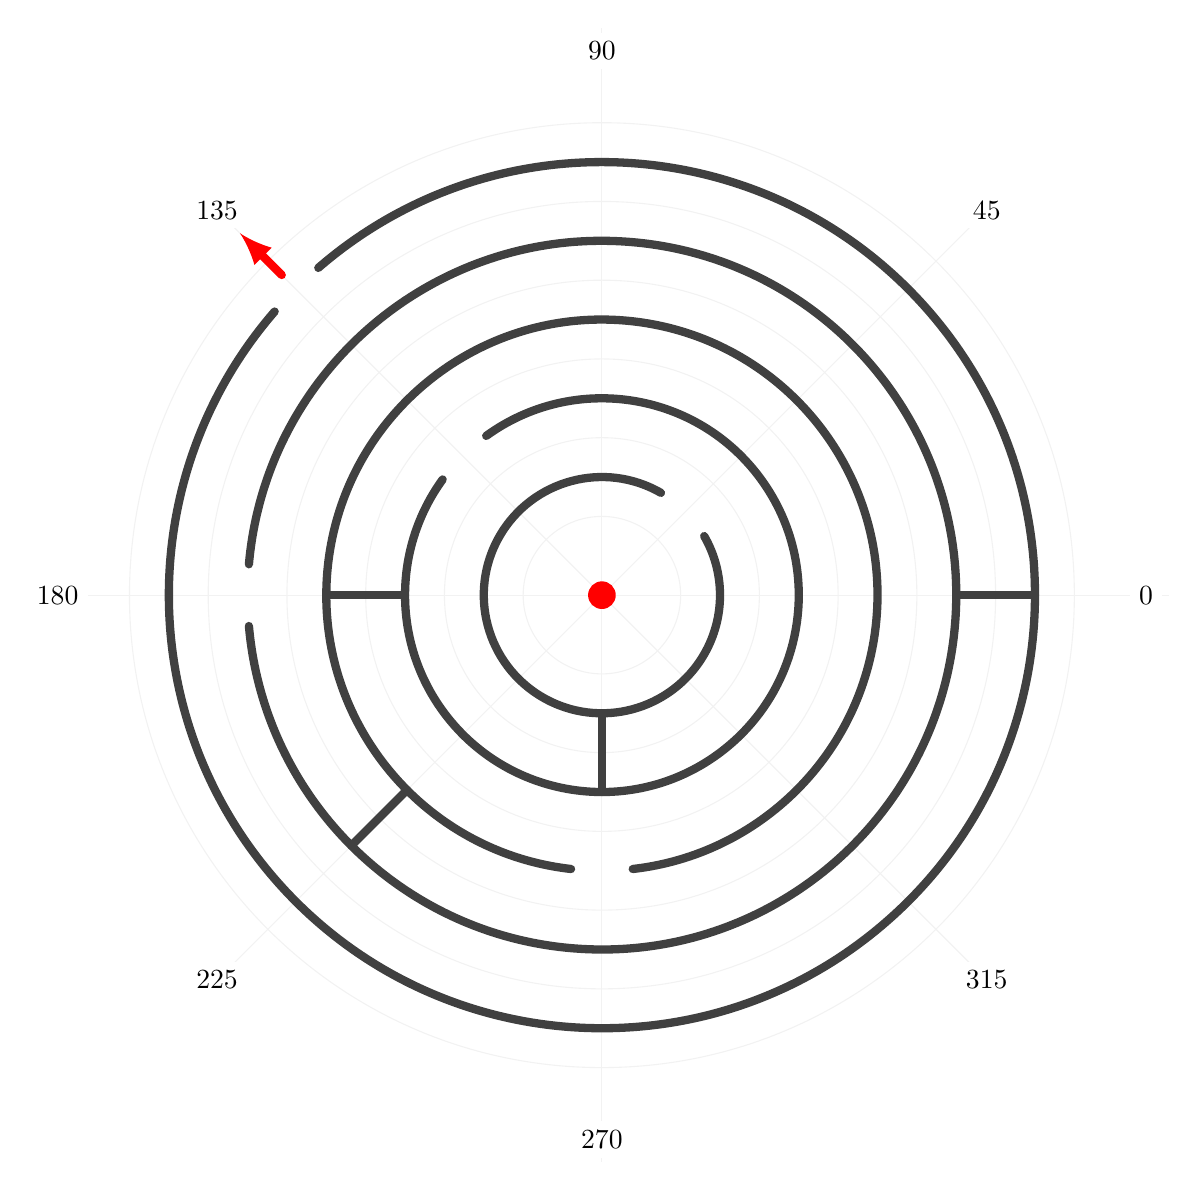
\begin{tikzpicture}

% Grid

\foreach \i in {1,2,...,6}
{
\draw[lightgray!20] (0,0) circle(\i);
}

\foreach \i in {0,45,90,135,...,315}
{
\draw[lightgray!20] (0,0) -- (\i:7.2) node[pos=0.96,black,fill= white]{\i};
}

% Puzzle

% circles
\begin{scope}[line width=3pt,cap=round, rounded corners=1pt,black!75]

\draw  (60:1.5) arc(60:390:1.5);

\draw  (126:2.5) arc(126:-216:2.5);

\draw  (263.575:3.5) arc(263.575:-83.575:3.5);

\draw  (175:4.5) arc(175:-175:4.5);

\draw  (130.91:5.5) arc(130.91:-220.91:5.5);

% Lines
\draw  (270:1.5) -- (270:2.5);
\draw  (180:2.5) -- (180:3.5);
\draw  (225:3.5) -- (225:4.5);
\draw  (0:4.5) -- (0:5.5);

\end{scope}


% Start and End Points
 \draw[-latex,line width=3pt,cap=round, rounded corners=1pt,red] (135:5.75)--(135:6.5);
 \fill[red] (0,0) circle(5pt);

\end{tikzpicture}

\end{document}